\chapter{Introdução}\label{cap:introducao}
Com o avanço dos computadores e das redes de comunicação, os sistemas de 
informação foram sendo transferidos dos computadores pessoais para os 
servidores \textit{web}, de onde eles podem ser acessados, virtualmente, a 
partir de todo o mundo. Para que esses sistemas funcionem, eles precisam de 
\textit{softwares} que atendam as requisições que chegam ao servidor a partir 
da rede de computadores usando o protocolo HTTP. Esses softwares são chamados 
servidores HTTP.\\
O aumento do uso de sistemas baseados na \textit{web} por organizações criou a 
necessidade de desenvolver aplicações que geram conteúdo dinamicamente. São 
essas aplicações que permitem as organizações entregar produtos, serviços e 
mensagens cujas formas e conteúdos são, em parte, determinadas pelas 
necessidades do usuário que será atendido.\\
Esse movimento para se afastar de conteúdos estáticos está levando ao limite e 
está expondo as fragilidades dos ambientes onde essas aplicações são 
executadas. Mais importante, esses ambientes não oferecem o desempenho que 
essas aplicações exigem. É preciso uma nova infraestrutura de comunicação para 
conectar servidores \textit{web} com essas novas aplicações.\\
De acordo com \citeonline{bondi2000}, escalabilidade é um atributo desejável de 
uma rede, sistema ou processo. O conceito tem a ver com a habilidade do sistema 
em acomodar uma quantidade sempre maior de elementos ou objetos, de processar 
uma quantidade crescente de trabalho de forma fácil e ou ser suscetível a 
ampliação. Quando estamos desenvolvimento um sistema, geralmente pede-se que 
ele seja escalável.\\
Quando se diz que um sistema não é escalável (ou que ele não escala), damos a 
entender que o custo adicional de lidar com o aumento em trafego ou tamanho é 
excessivo, ou que o sistema não consegue lidar com esse nível elevado de 
acesso. O custo pode ser quantificado de várias formas, incluindo mas não 
limitado à tempo de resposta, uso de processamento, espaço, memória e até mesmo 
dinheiro. Um sistema que não escala bem adiciona custos de manutenção ou 
danifica a qualidade do serviço, pode atrasar ou privar o usuário de 
oportunidades de lucro e eventualmente ele precisará ser substituído.\\
A escalabilidade de um sistema sujeito a crescimento é crucial para o seu 
sucesso a longo prazo. Ao mesmo tempo, o conceito de escalabilidade e o nosso 
entendimento dos fatores que aumentam ou diminuem são vagos e até mesmo 
subjetivos. Desenvolvedores de sistemas e analistas de desempenho tem um 
sentimento intuitivo sobre escalabilidade, mas os fatores determinantes não são 
claros e podem variar de um sistema para outro.\\
A escalabilidade de um sistema pode ser arruinado por desperdícios herdados de 
ações repetidas de forma frequente. Também pode ser arruinado pela presença de 
algoritmos de acesso que levam a \textit{deadlock} ou que resultam em um 
escalonamento ruim de recursos. Tais sistemas podem funcionar bem quando a 
carga está baixa, mas sofrer uma degradação substancial de desempenho quando a 
carga aumenta.\\
Hoje, na UFVJM, é utilizado o SIGA – Sistema Integrado de Gestão Acadêmica, 
comprado em 2.007 da Universidade Federal de Juiz de Fora.O SIGA é desenvolvido 
utilizando a linguagem de programação PHP e o \textit{framework} Miolo e 
utiliza o Apache HTTP \textit{Server} como servidor HTTP e o PostgreSQL como 
SGBD.\\
O Apache, desde 1.995 tem sido o servidor HTTP mais utilizado no mundo. Em 
Outubro de 2.014, de acordo com pesquisa realizada em 1.028.932.208 de sítios 
pela empresa Netcraft, o Apache era usado por 37,79\% (385.354.994) desses 
sítios, com o Microsoft IIS aparecendo em segundo com 33,58\% (345.485.419) e o 
Nginx em terceiro com 14,42\% (148.330.190) de participação nos sítios, como 
visto na figura \ref{fig:webservers-utilizacao}.\\
Nessa mesma pesquisa, entre os 1 milhão de sites mais acessados no mundo, o 
Apache é utilizado em 50,19\% (501,922), com o Nginx em segundo lugar com 
14,36\% (25,588,943), como visto na figura 
\ref{fig:webservers-utilizacao-milhao}\\.
\begin{figure}[htb]
	\centering
	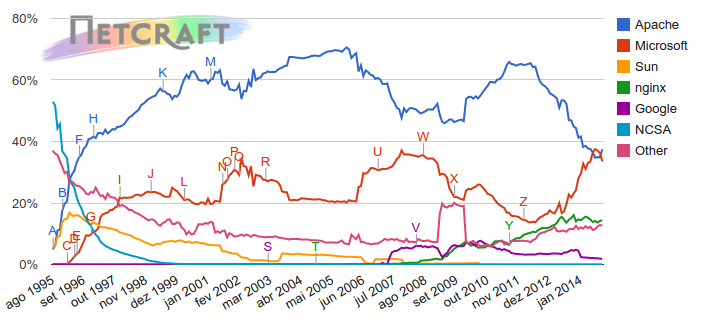
\includegraphics[width=1\linewidth]{figuras/grafico1}
	\caption{Utilização de Servidores \textit{web} no mundo.}
	\label{fig:webservers-utilizacao}
\end{figure}

\begin{figure}[htb]
	\centering
	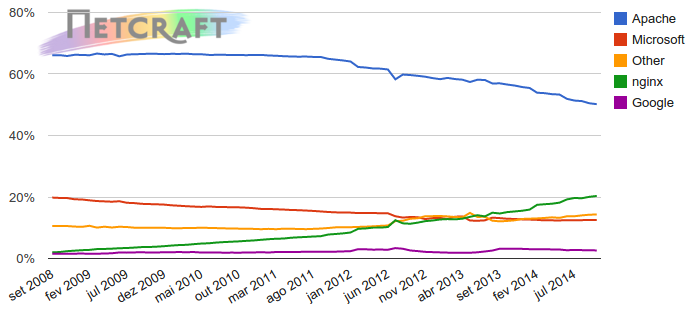
\includegraphics[width=1\linewidth]{figuras/grafico2} 
	\caption{Utilização de Servidores \textit{web} entre os 1.000.000 de sítios 
	mais acessados no mundo.}
	\label{fig:webservers-utilizacao-milhao}
\end{figure}
Analisando os gráficos presentes nas figuras \ref{fig:webservers-utilizacao} e 
\ref{fig:webservers-utilizacao-milhao}, é possível notar uma queda na 
utilização do Apache em detrimento de outros servidores HTTP, sendo mais 
notório a queda na utilização entre os 1 milhão de sítios mais acessados. É 
possível notar também o aumento no uso do Nginx, principalmente entre os 1 
milhão de sítios mais acessados no mundo. É necessário frisar que só porque uma 
tecnologia está em ascensão significa que ela é melhor, mais é necessário 
investigar os motivos pelo qual tal tecnologia está crescendo em número de 
utilizadores.\\
Tendo sido desenvolvidos em épocas diferentes, o Apache e o Nginx trabalham de 
forma diferente na hora de atender as requisições HTTP que chegam ao servidor.\\
De acordo com \citeonline{rowe}, o Apache cria processos e \textit{threads} 
para lidar com as requisições, ficando a cargo do administrador do servidor a 
tarefa de configurar o Apache para controlar o numero máximo de processos e 
\textit{threads} permitidos. Muitas \textit{threads} podem exaurir a memória 
principal(RAM) e pode forçar o servidor a usar memória \textit{SWAP}, 
degradando severamente o desempenho. Além disso, quando chega ao limite de 
processos, o Apache passa a recusar conexões.
\section{Motivação}
De acordo com o Plano de Desenvolvimento Institucional para o ciclo 2.012 - 
2.016 da UFVJM, além dos quatro \textit{campi} já implantados (Diamantina, 
Teófilo Otoni, Janaúba e Unaí) o existe o projeto para a implantação de outros 
quatro \textit{campi} universitários nas cidade de Capelinha, Araçuaí, Almenara 
e Nanuque, totalizando oito \textit{campi} espalhados pelas regiões Norte, 
Noroeste, Vales do Jequitinhonha e Mucuri do estado de Minas Gerais. O 
PDI 
contempla também a ampliação da oferta de vagas para cursos de graduação nos 
\textit{campi} Diamantina e Teófilo Otoni.
Com a expansão das Universidades Federais através do programa REUNI, por ano 
são admitidos 3500 alunos de graduação, pós-graduação e educação à distância 
além de novos servidores técnicos-administrativos e professores. Somente no 
último edital para seleção de técnicos-administrativos, foram oferecias 148 
vagas.\\
Em julho de 2.014, data do último levantamento, a Universidade Federal dos 
Vales do Jequitinhonha e Mucuri tinha 8.121 alunos, 576 professores e 421 
servidores técnicos-administrativos, espalhados em quatro \textit{campi} 
universitários, fazendas experimentais e pólos de ensino em educação à 
distância, totalizando 9.118 pessoas que interagem com a universidade 
diariamente.\\
Em épocas de pico de utilização do SIGA, as reclamações de lentidão e problemas 
no sistemas são frequentes, as vezes impossibilitando a utilização do mesmo. Os 
picos mais notório são: fim de período letivo da graduação, quando alunos e 
professores acessam o sistema para olhar e lançar notas, respectivamente; e 
rematricula dos alunos da graduação, quando os mesmos escolhem as matérias que 
desejam cursar no período seguinte.\\
Com o crescente aumento de alunos, servidores públicos (professores e técnicos-administrativos) e teceirizados na universidade, a tendência é que a utilização do SIGA se torne mais problemática.
Com isso em mente, a utilização do servidor HTTP Nginx pode ajudar a amenizar 
os problema de desempenho do SIGA.\\
\section{Objetivos}
Identificar se a utilização do servidor HTTP Nginx é mais eficiente do que o 
utilizado atualmente, o Apache HTTP \textit{Server}.\\
\section{Objetivos específicos}
Analisar os dados coletados a partir de testes realizados para identificar se o 
Nginx é mais eficiente do que o Apache; apresentar a solução encontrada e 
analisar o que pode ser feito para evitar a substituição ou reconstrução do 
SIGA.\\
\section{Organização do trabalho}
O trabalho está organizado em oito capítulos, sendo essa introdução o primeiro. 
O capítulo \ref{cap:fundamentacao-teorica}, será exposto toda a teoria por trás 
do estudo feito. No capítulo \ref{cap:tecnologias_utilizadas}, serão descritos 
os programas e ferramentas utilizados implicitamente e explicitamente nos 
testes. No capítulo \ref{cap:metodologia} será descrito como os testes foram 
realizados e quais dados foram coletados e descrever os ambientes onde foram 
feitos os teste de desempenho do Apache e do Nginx. No capítulo 
\ref{cap:analise-dos-dados} os dados serão apresentados e 
será feita uma análise sobre o desempenho dos dois servidores HTTP. E 
finalmente, no capítulo \ref{cap:conclusao} eu apresentarei as minhas 
conclusões sobre o estudo.\\
